\section{Sequence Diagrams}
To clarify the interactions between user and system components, we provide sequence diagrams for the five main use cases.

\subsection{Sequence Diagram for Uploading a Video}
Figure \ref{fig:uc1_seq} illustrates the process of uploading a video lecture. The user initializes the upload, and the Video Service validates the file format. Upon success, the file is stored in MinIO object storage, and a transcription job is enqueued in Redis for async processing.

\begin{figure}[H]
    \centering
    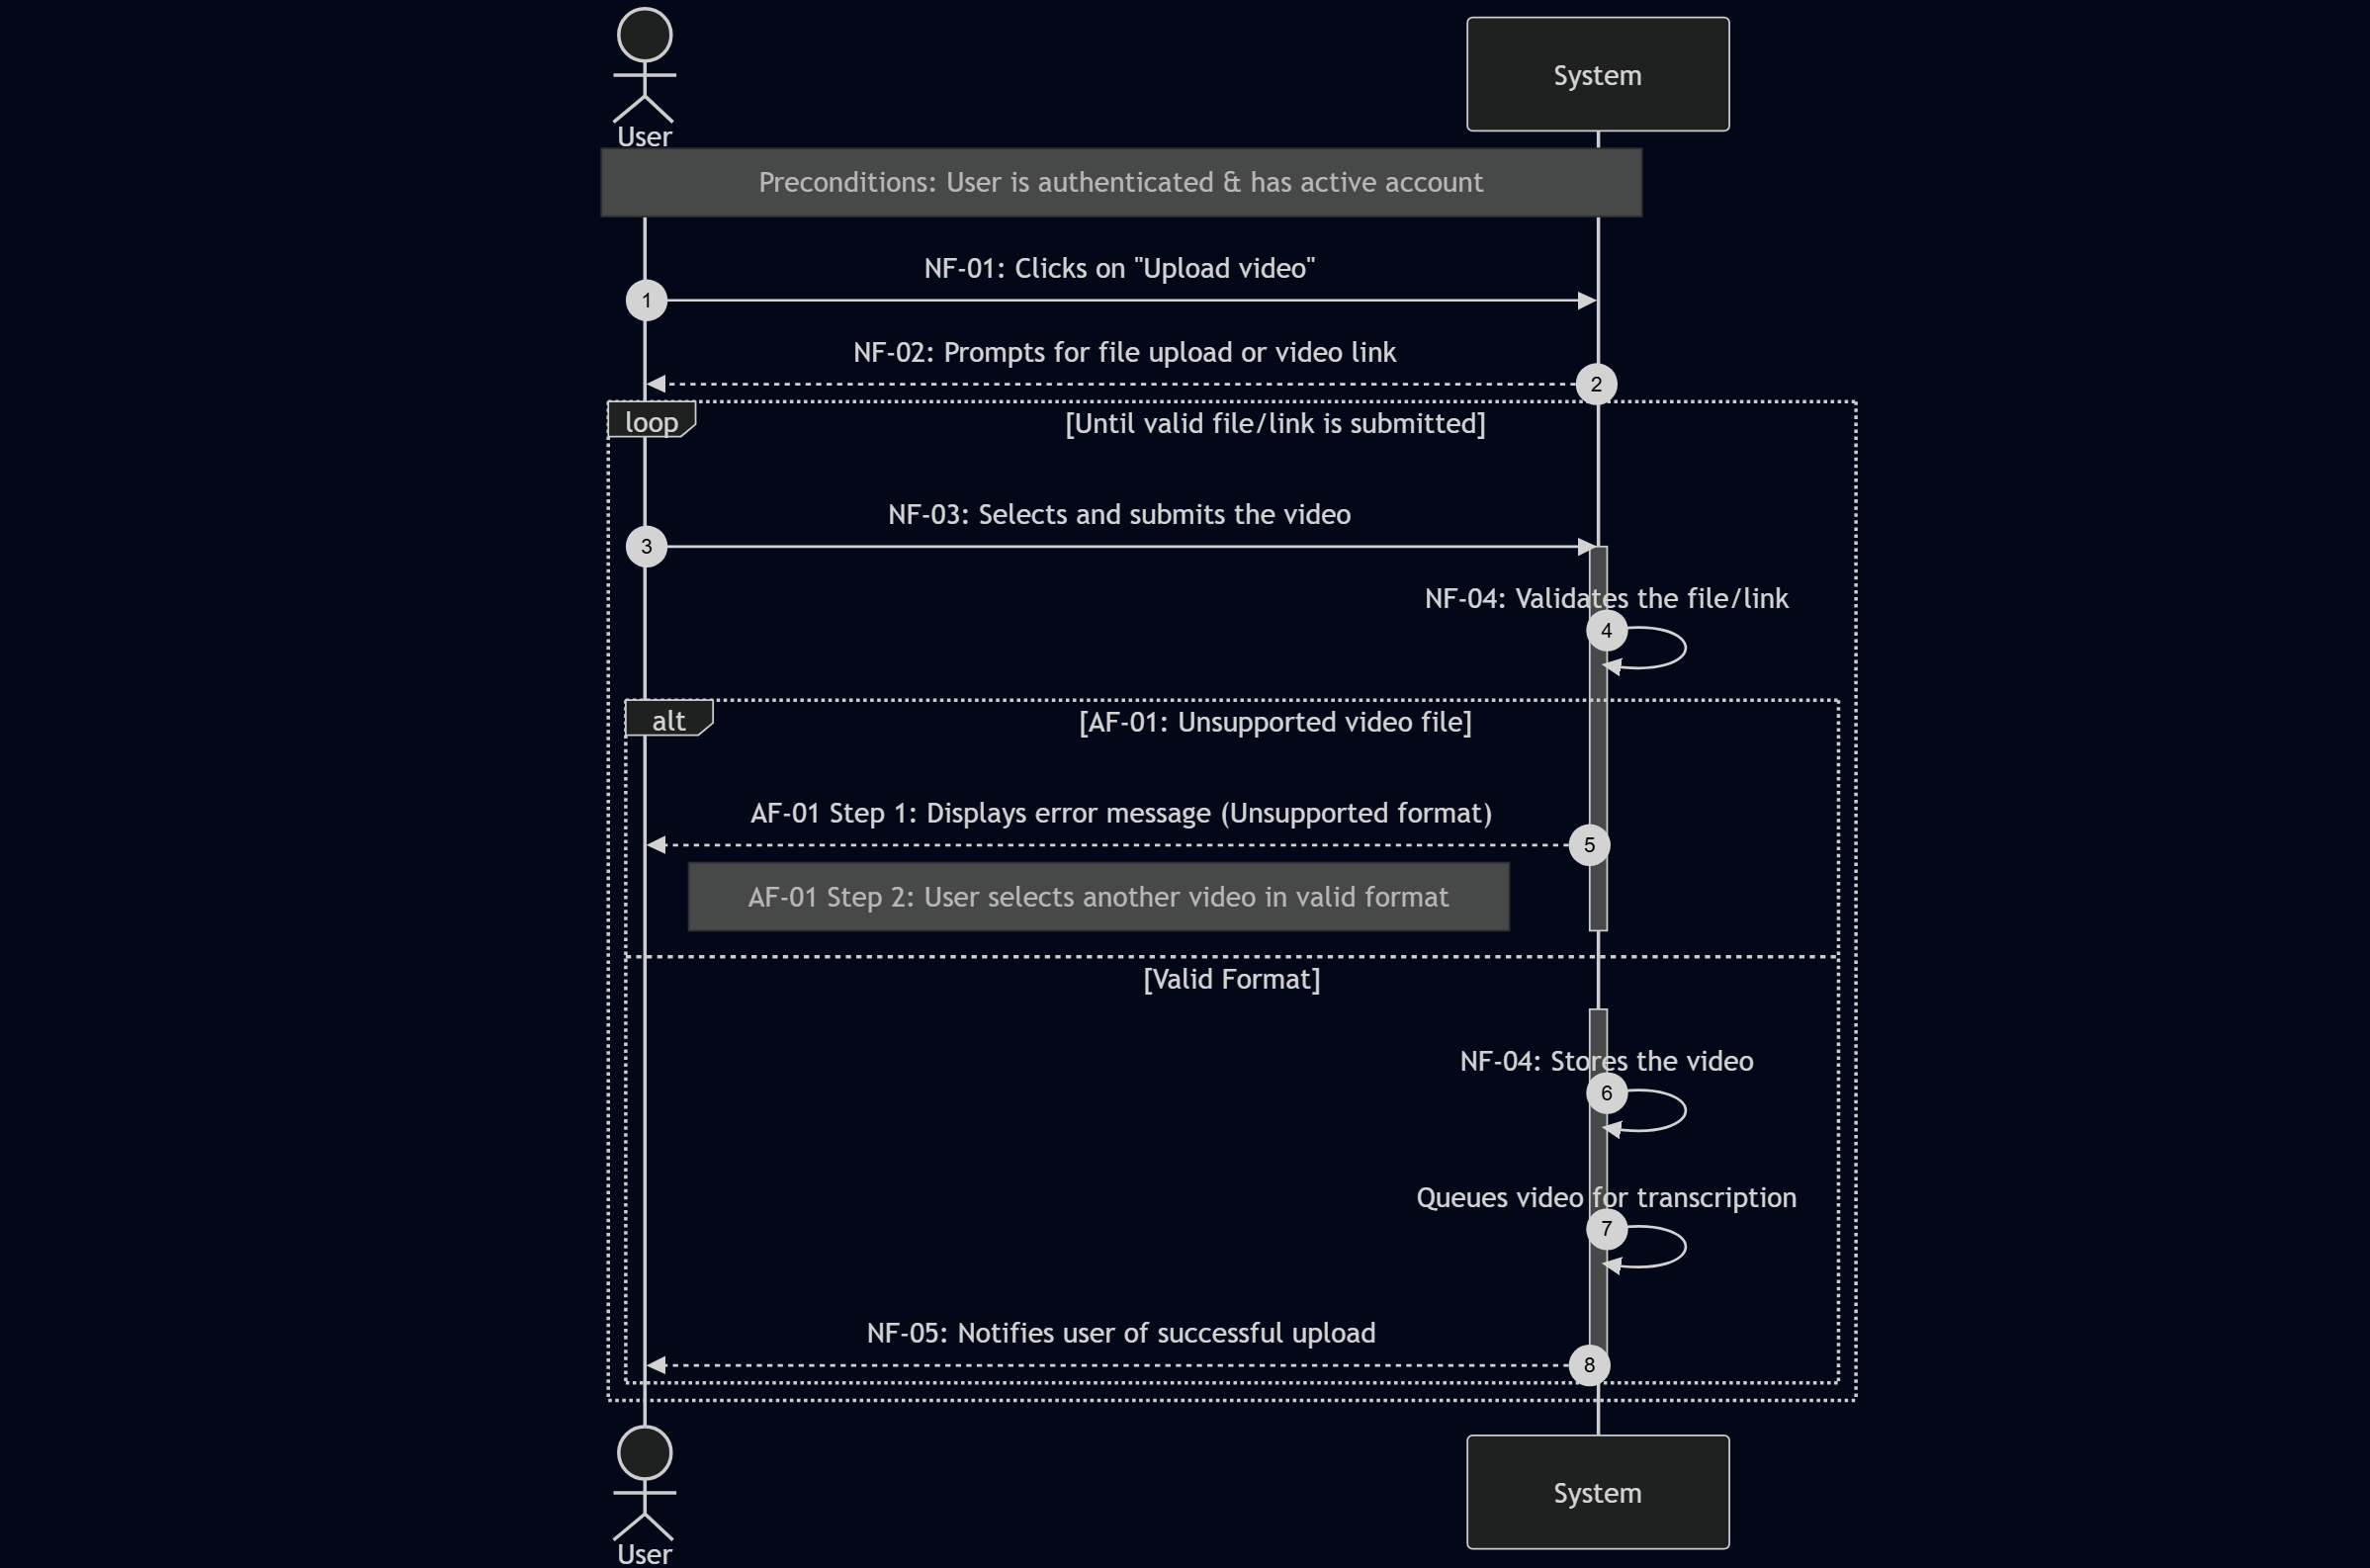
\includegraphics[width=1.0\linewidth]{system/images/UC1.png}
    \caption{Sequence Diagram: Upload Video (UC-01)}
    \label{fig:uc1_seq}
\end{figure}

\subsection{Sequence Diagram for Video Summarization}
After the transcription is complete, the user can request a summary. As shown in Figure \ref{fig:uc2_seq}, the Summarization Service retrieves the full transcript from MongoDB, processes it through the Pegasus AI model to generate an abstractive summary, and returns the result to the user.

\begin{figure}[H]
    \centering
    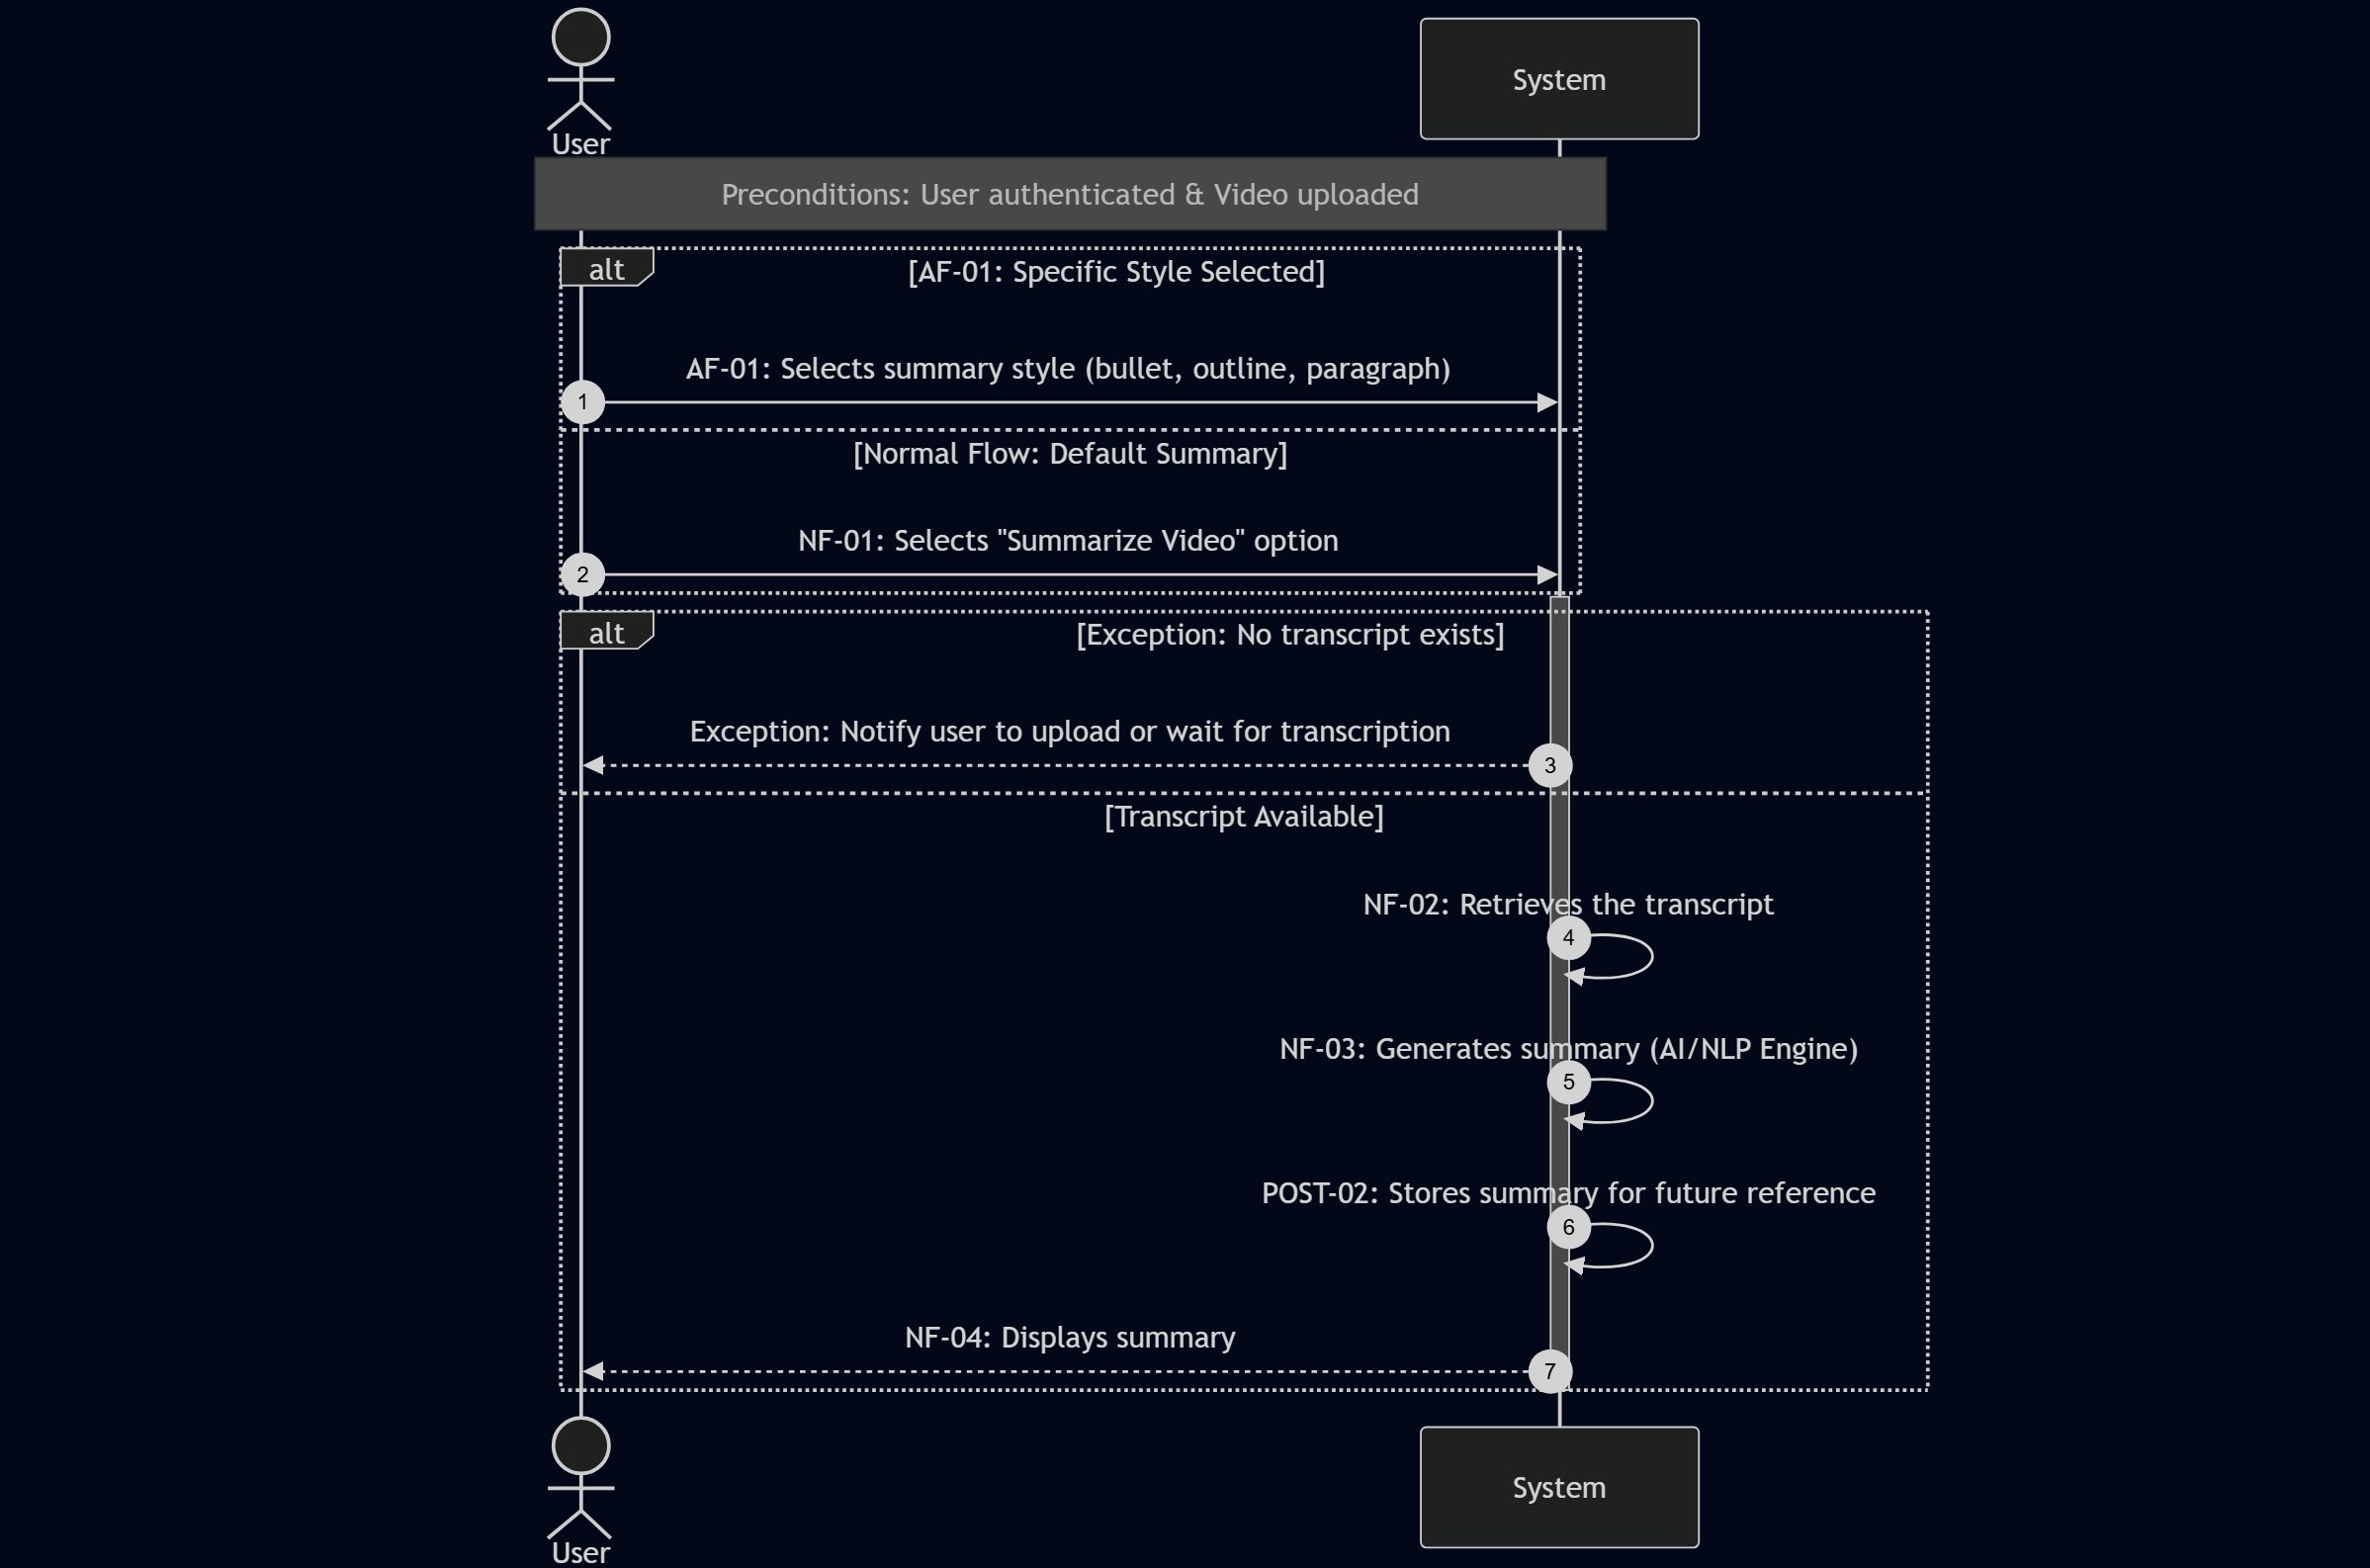
\includegraphics[width=1.0\linewidth]{system/images/UC2.png}
    \caption{Sequence Diagram: Summarize Video (UC-02)}
    \label{fig:uc2_seq}
\end{figure}

\subsection{Sequence Diagram for Quiz Generation}
Figure \ref{fig:uc3_seq} depicts the flow for generating assessments. The Quiz Service uses the Flan-T5 model to analyze the transcript content and generate a set of multiple-choice questions. These questions are then stored in the MySQL database for later retrieval.

\begin{figure}[H]
    \centering
    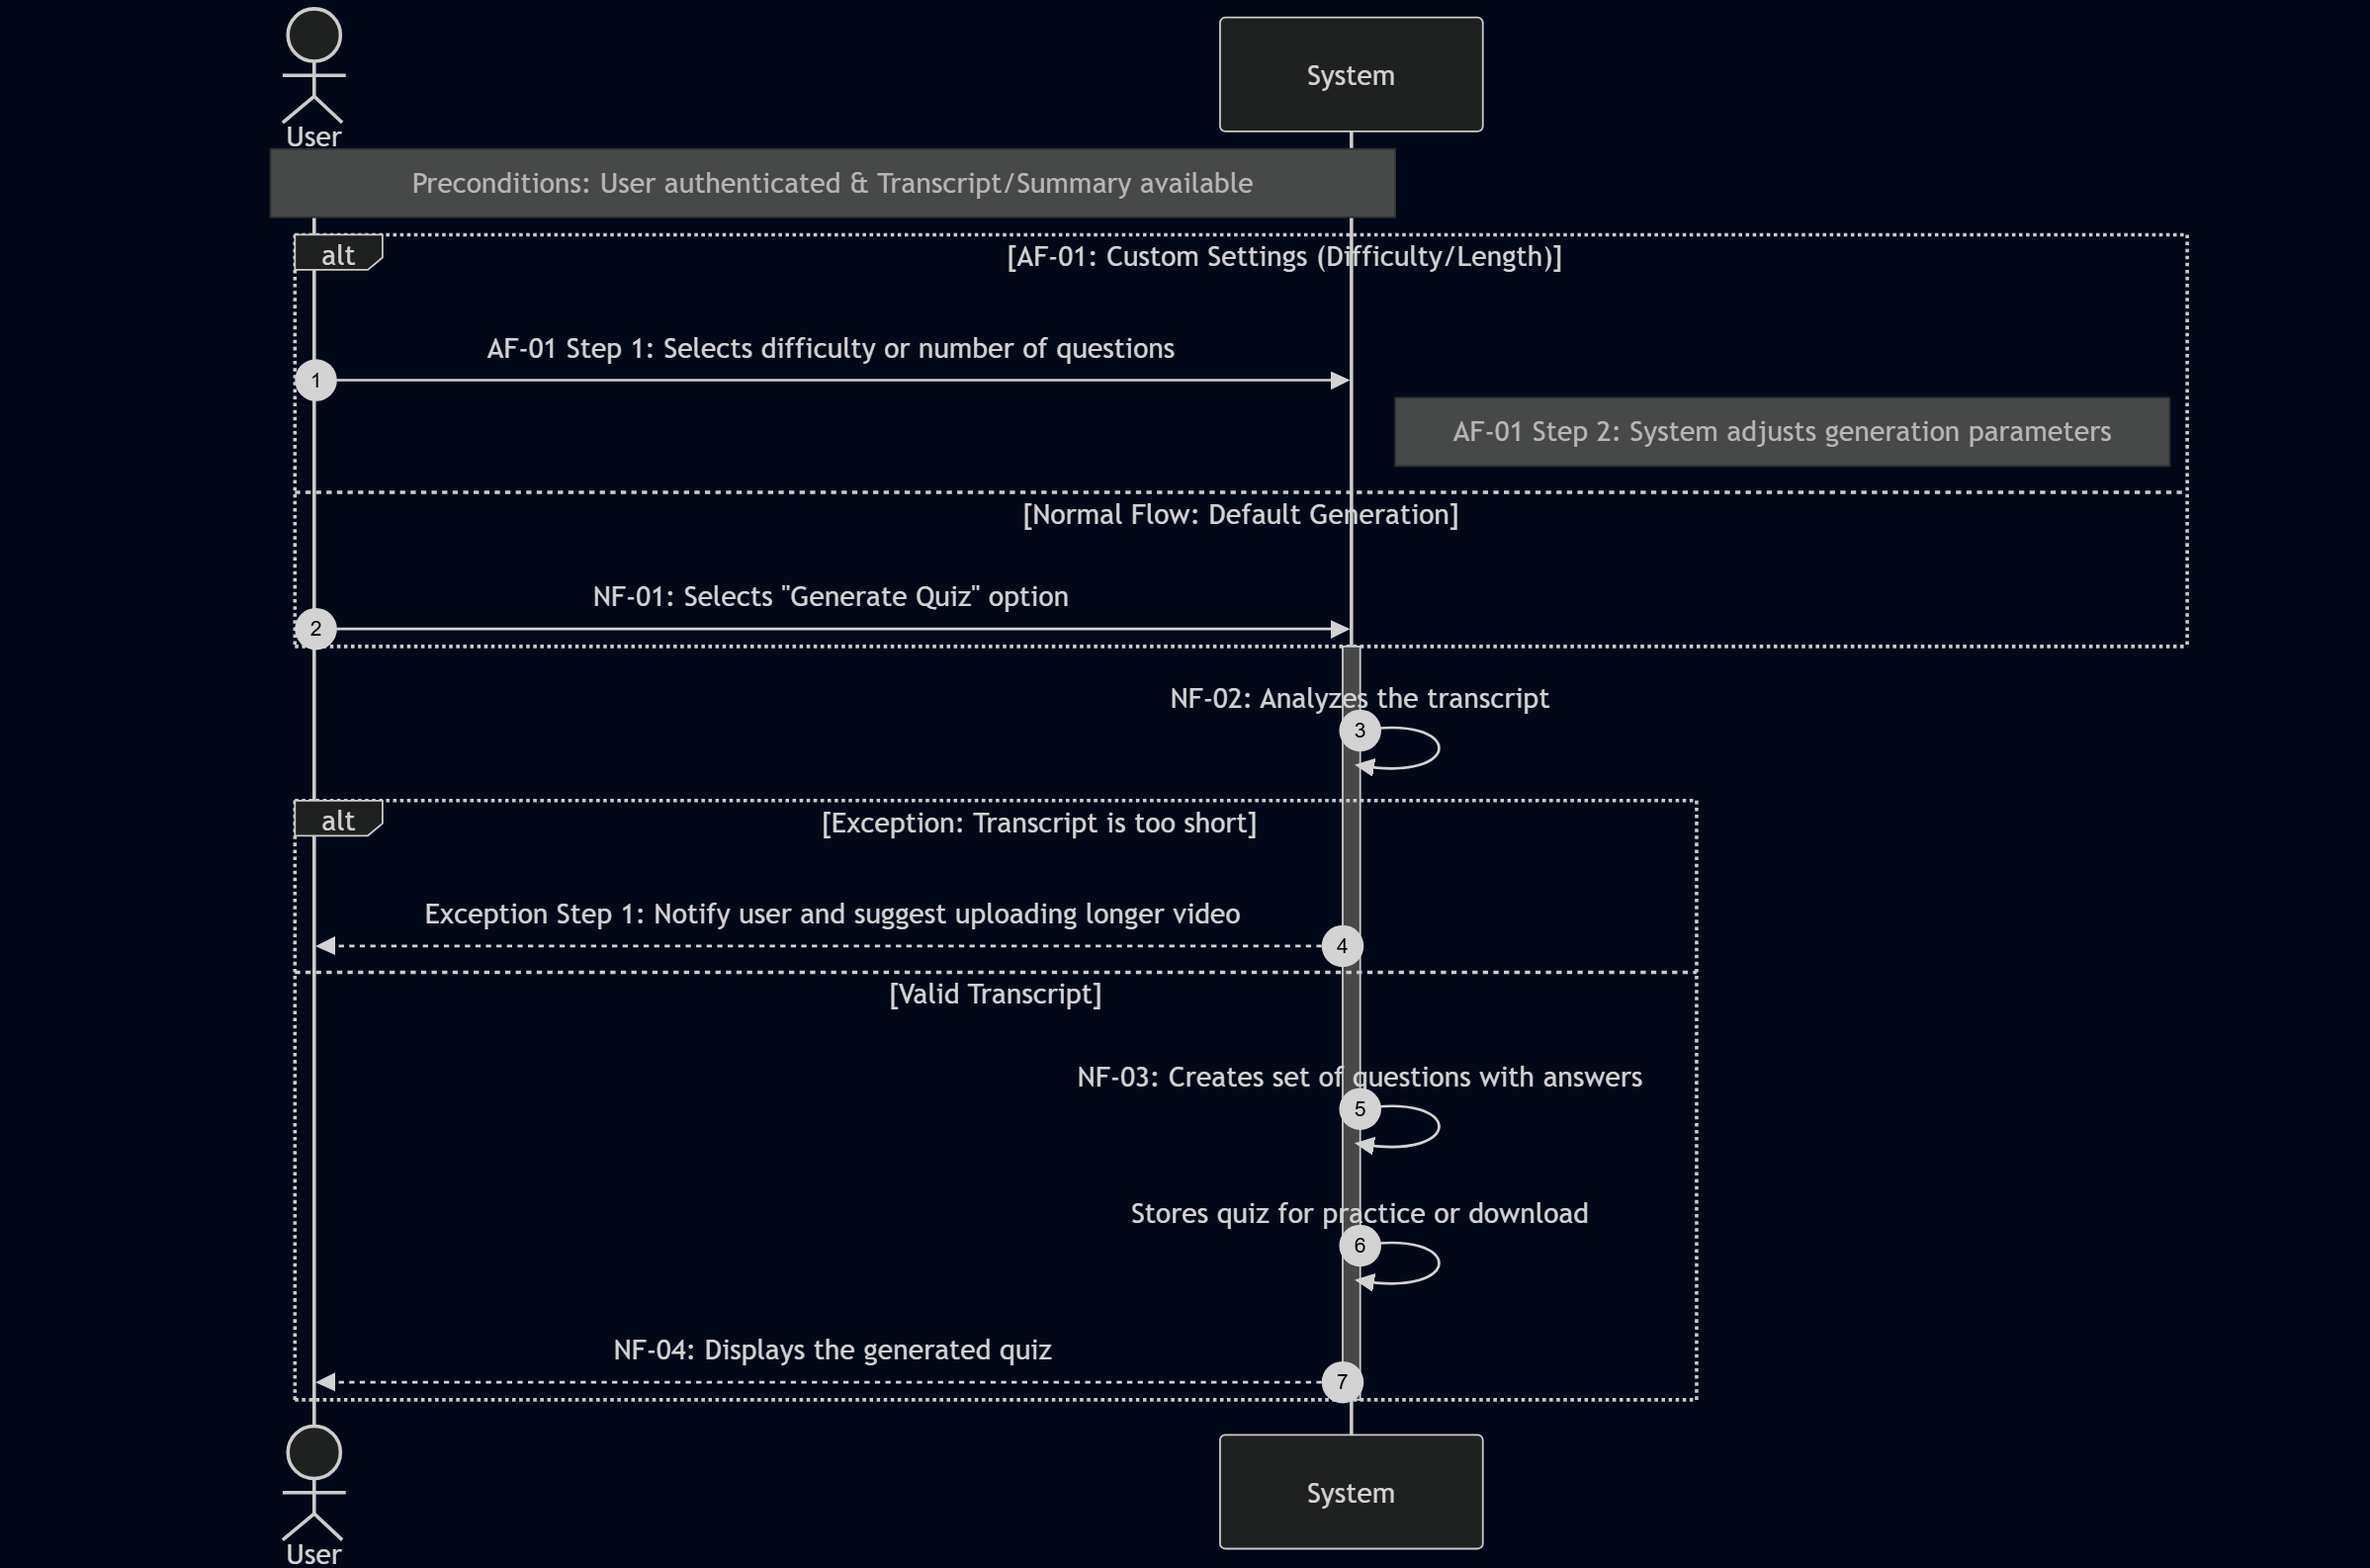
\includegraphics[width=1.0\linewidth]{system/images/UC3.png}
    \caption{Sequence Diagram: Generate Quiz (UC-03)}
    \label{fig:uc3_seq}
\end{figure}

\subsection{Sequence Diagram for Taking a Quiz}
When a user attempts a quiz, the system retrieves the questions and presents them interactively (Figure \ref{fig:uc4_seq}). The user's answers are evaluated in real-time or upon completion, providing immediate feedback and calculating a final score which is recorded in the user's history.

\begin{figure}[H]
    \centering
    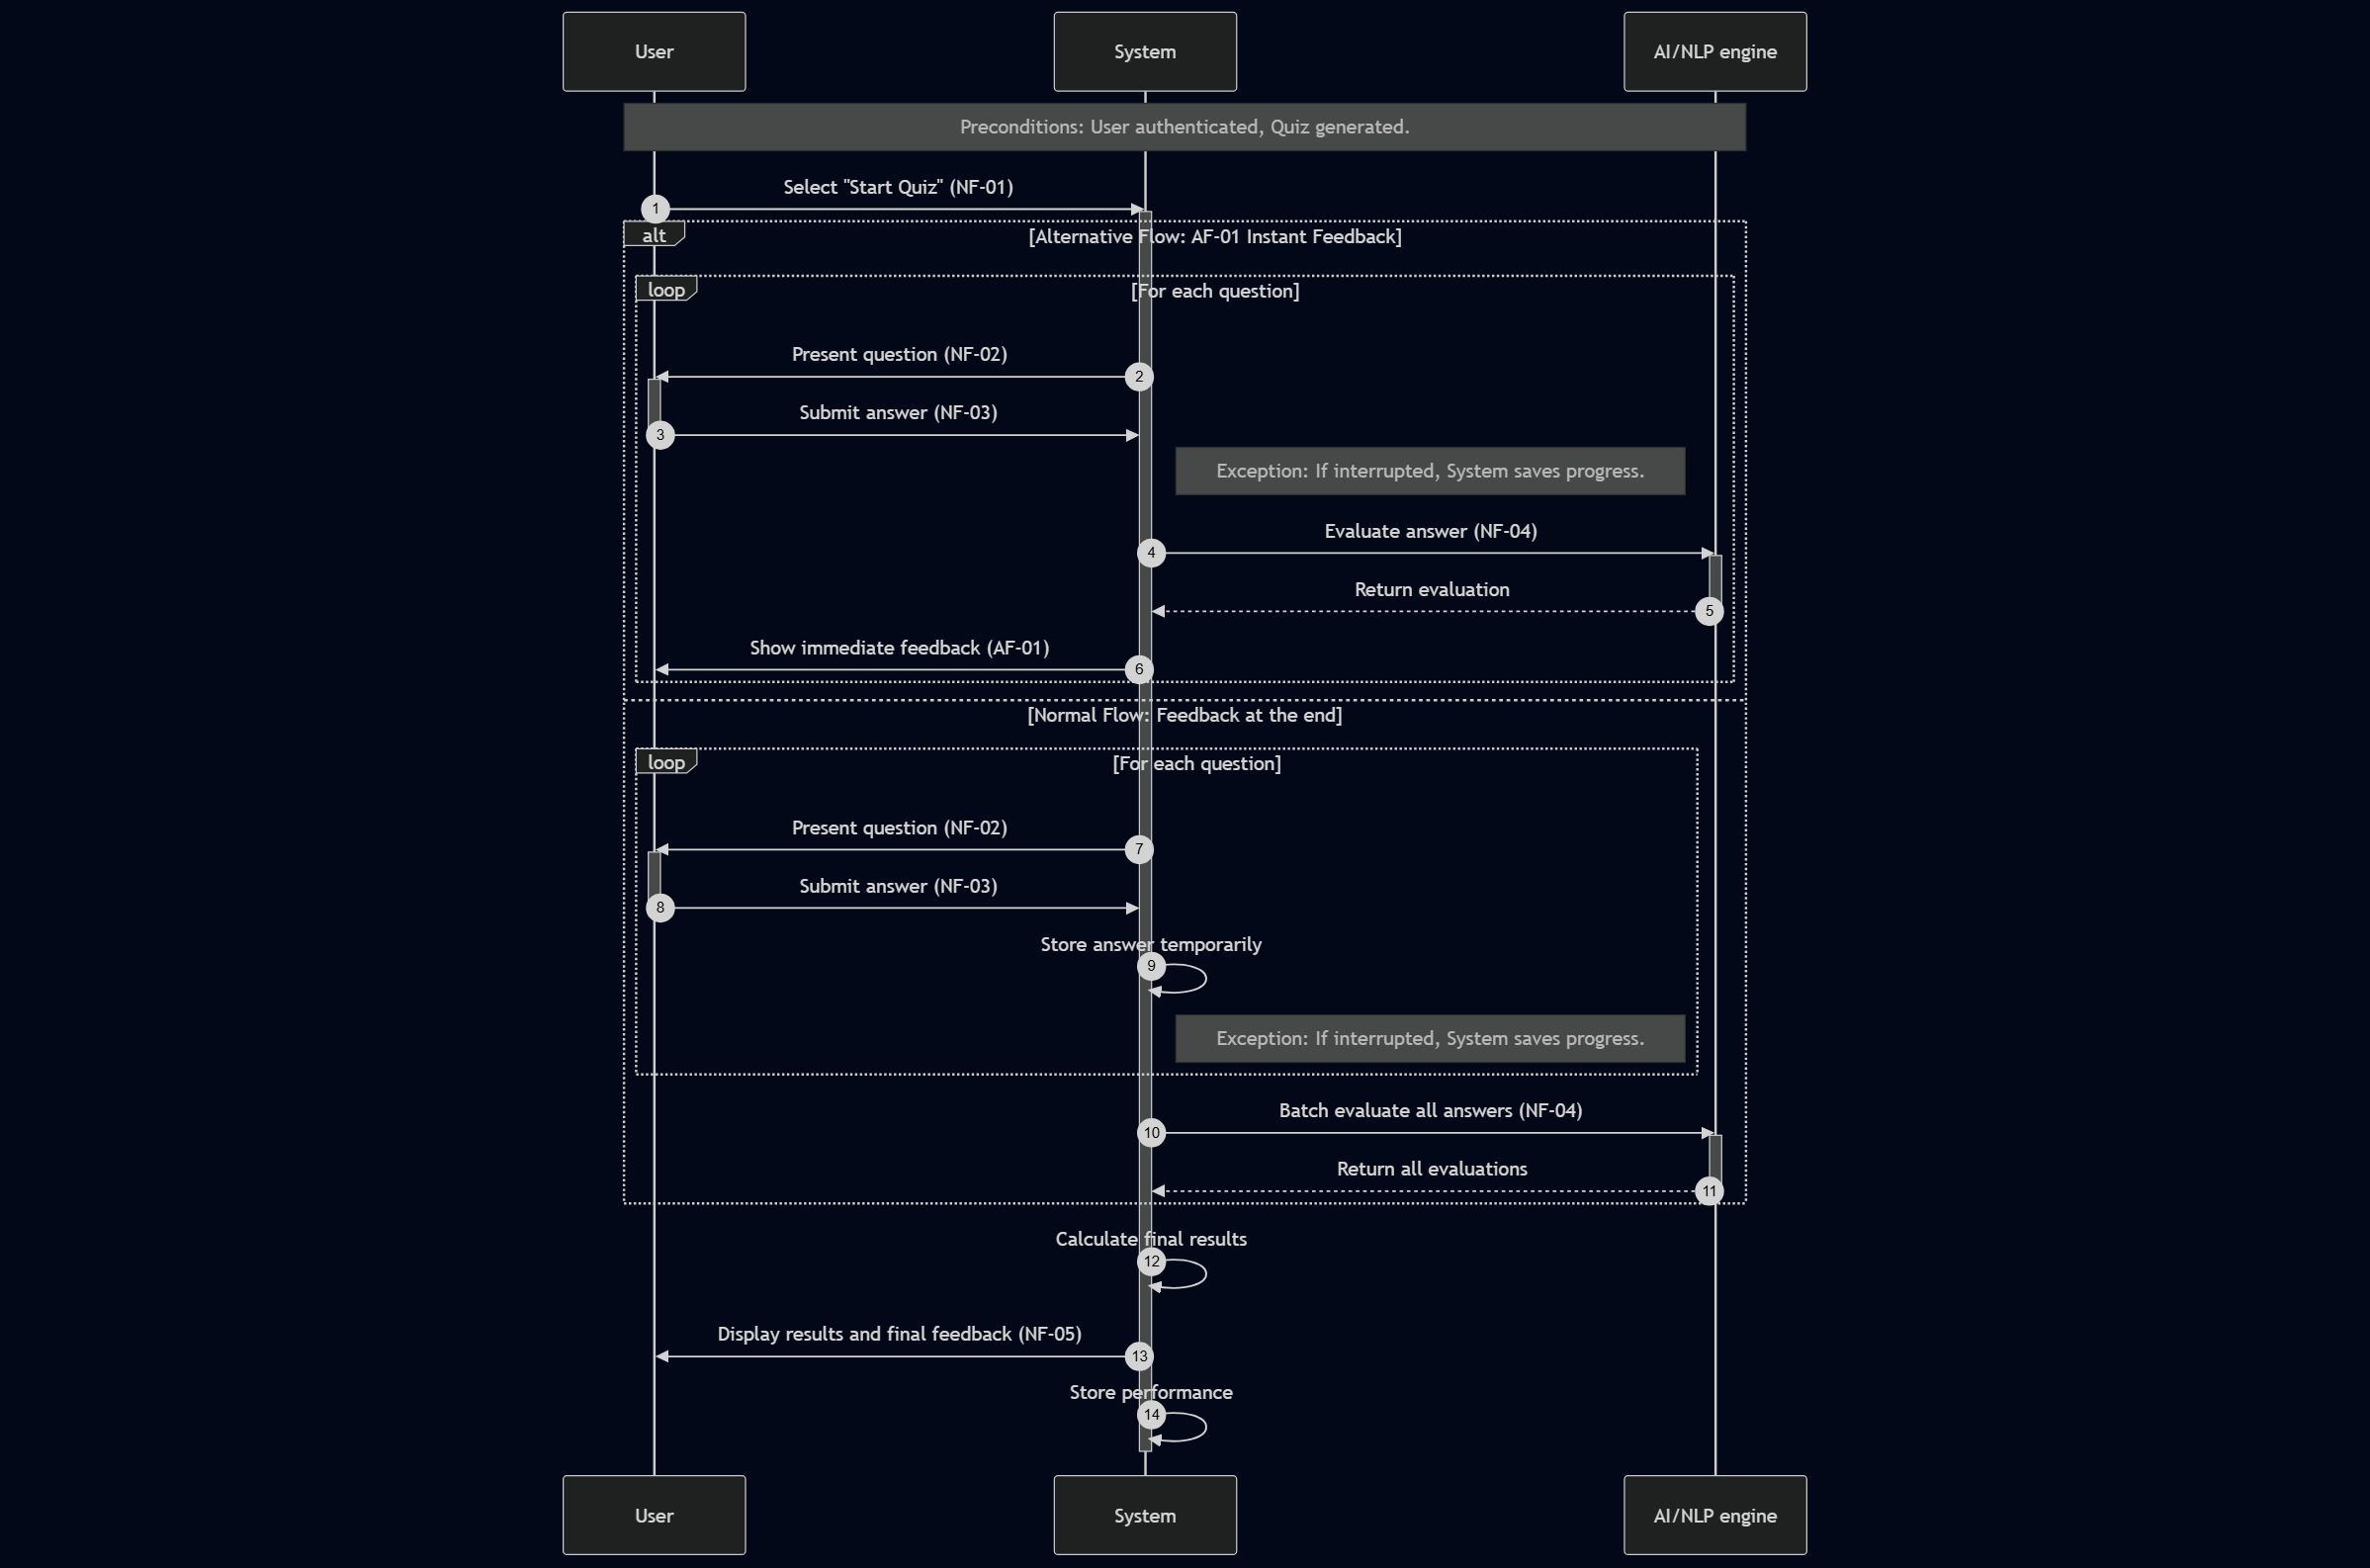
\includegraphics[width=1.0\linewidth]{system/images/UC4.png}
    \caption{Sequence Diagram: Take Quiz \& Get Feedback (UC-04)}
    \label{fig:uc4_seq}
\end{figure}

\subsection{Sequence Diagram for Results Export}
The final diagram (Figure \ref{fig:uc5_seq}) shows the export workflow. Users can choose to download their summaries, quiz results, or full transcripts. The system compiles the requested data into the selected format (PDF, DOCX) and generates a downloadable file.

\begin{figure}[H]
    \centering
    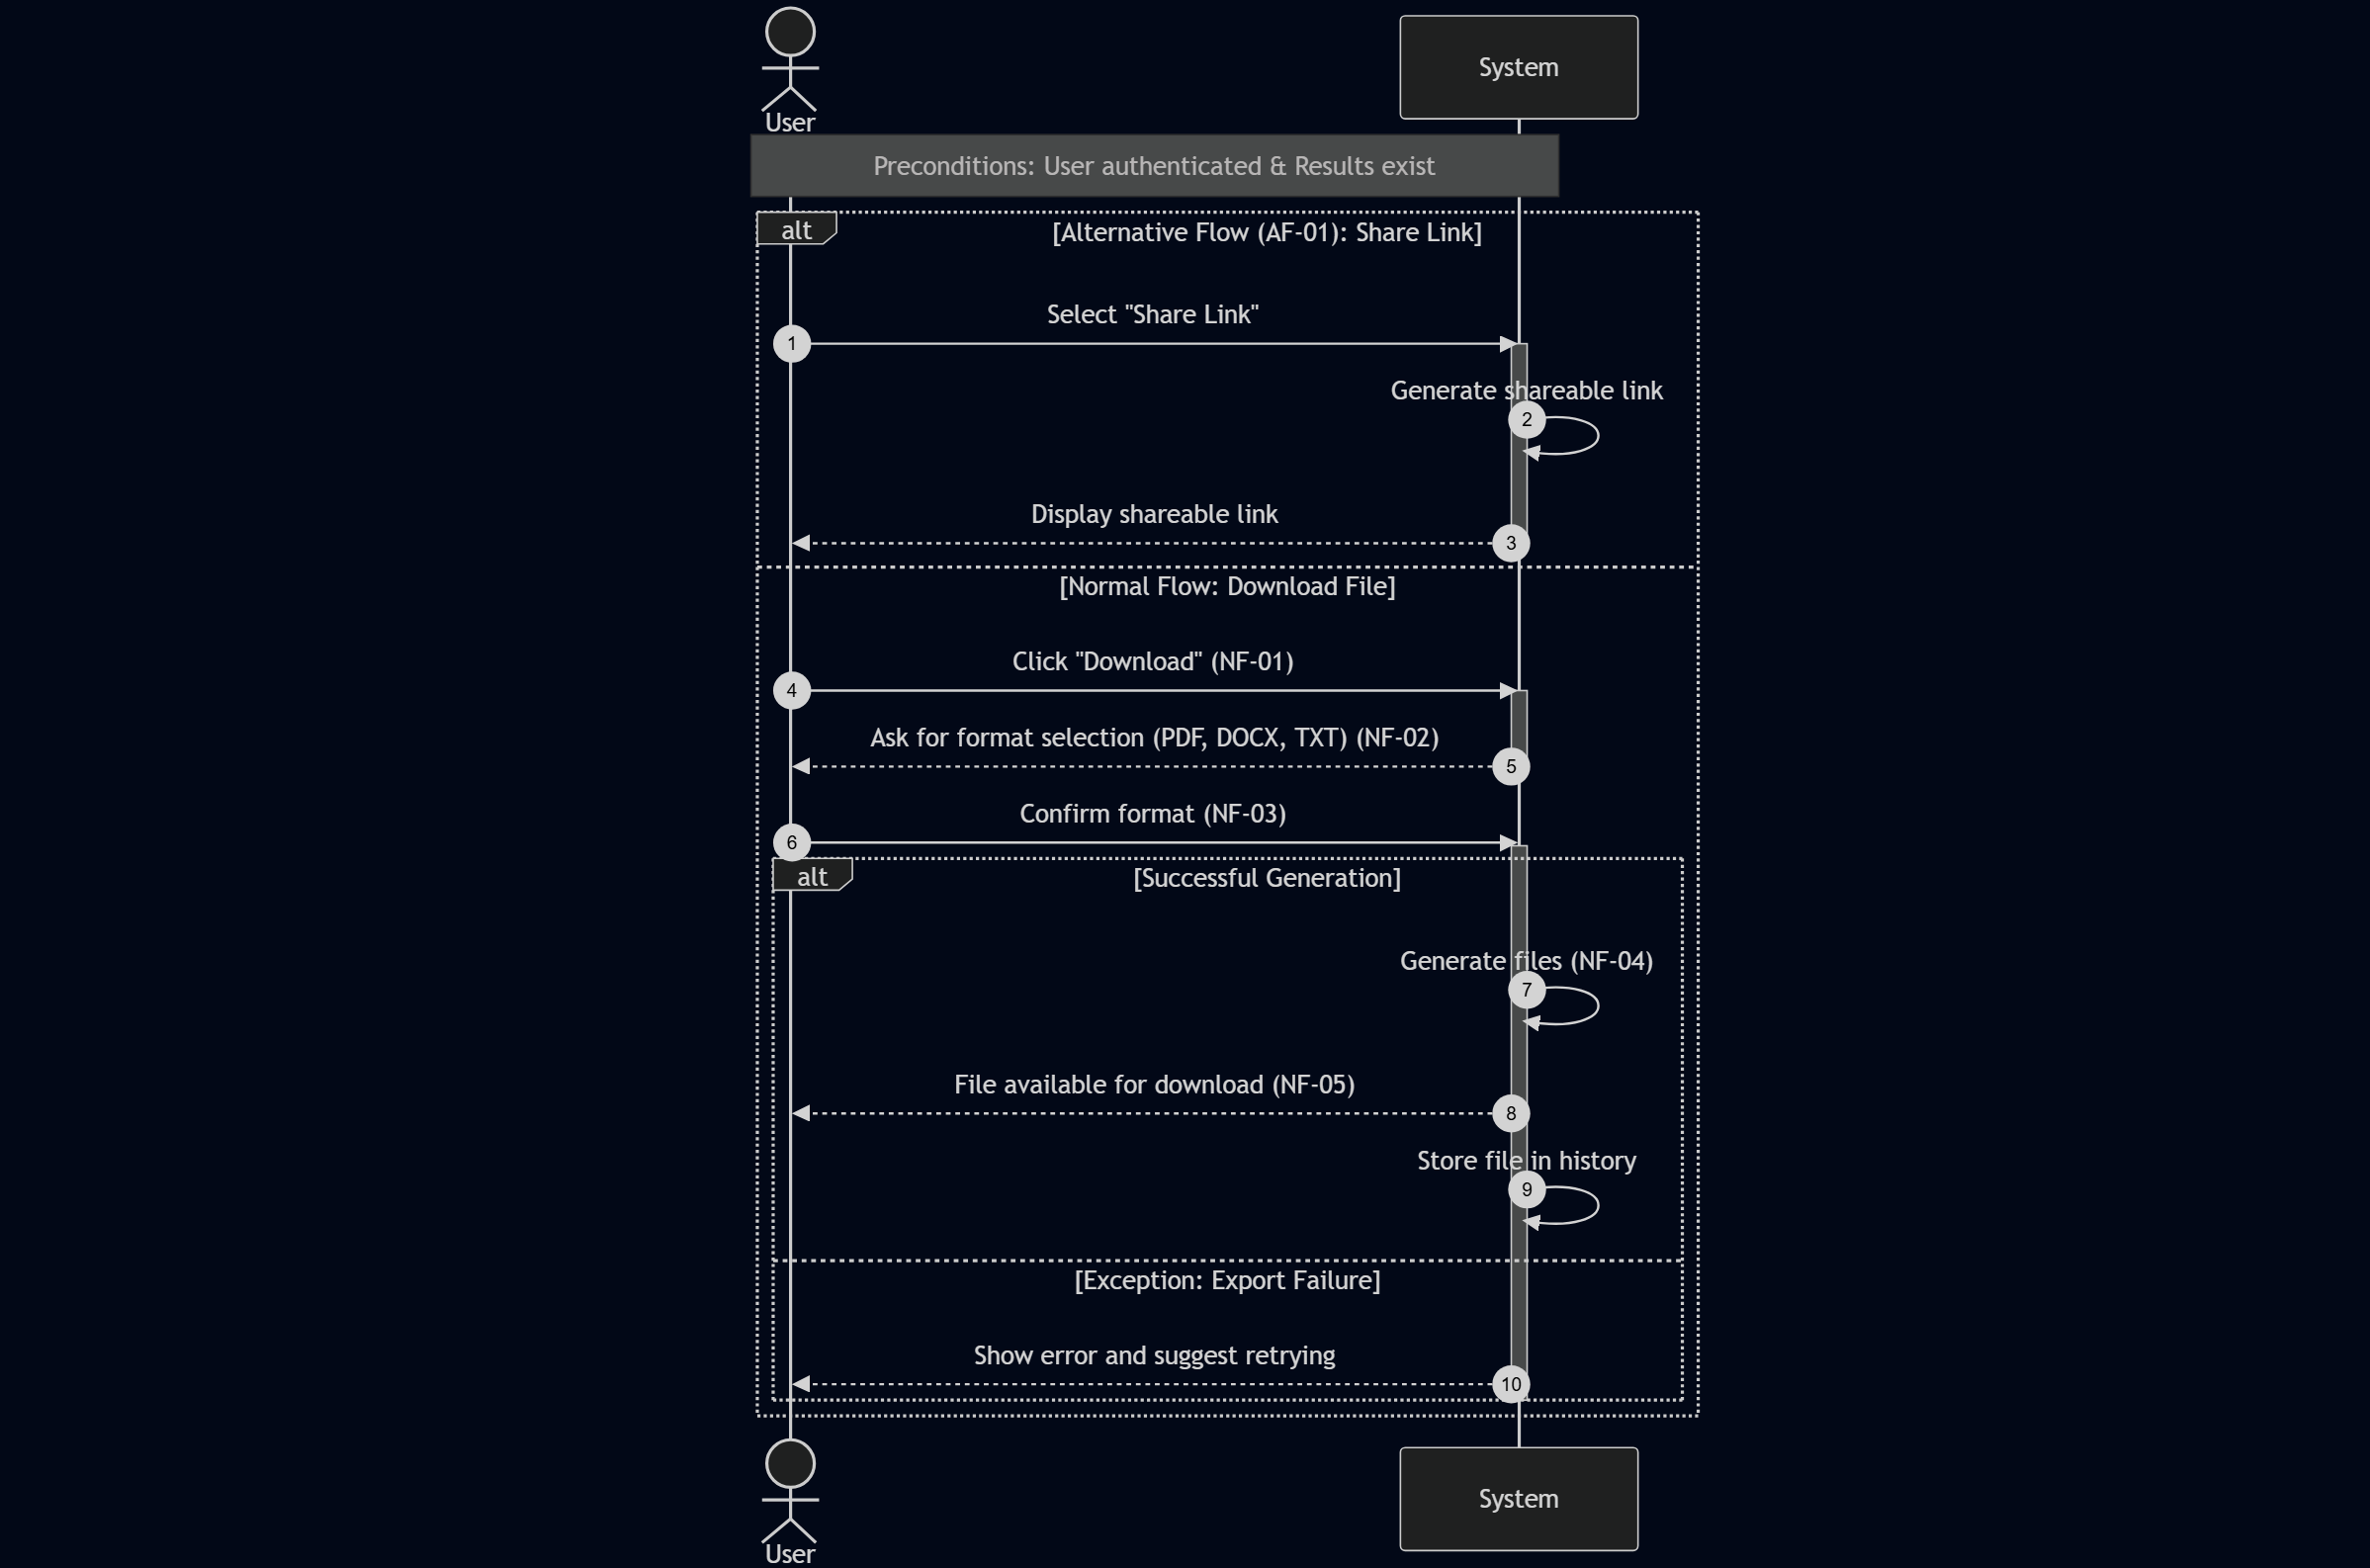
\includegraphics[width=1.0\linewidth]{system/images/UC5.png}
    \caption{Sequence Diagram: Download/Export Results (UC-05)}
    \label{fig:uc5_seq}
\end{figure}
